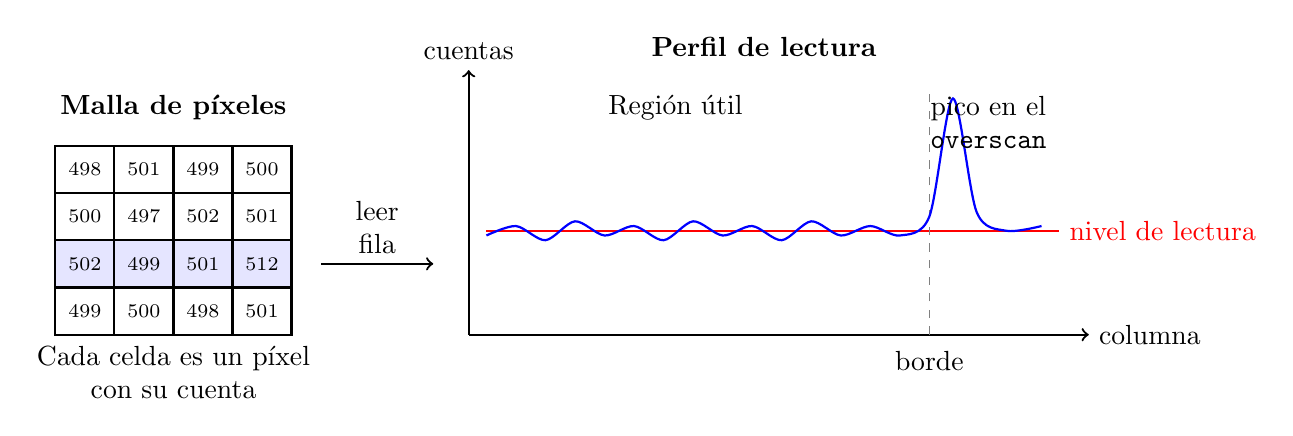
\begin{tikzpicture}[x=0.75cm,y=0.6cm]
  \node[font=\bfseries] at (2,4.8) {Malla de píxeles};
  \fill[blue!10] (0,1) rectangle (4,2);
  \draw[thick] (0,0) rectangle (4,4);
  \foreach \gridline in {1,2,3} {
    \draw[thick] (\gridline,0) -- (\gridline,4);
    \draw[thick] (0,\gridline) -- (4,\gridline);
  }
  \node[font=\scriptsize] at (0.5,3.5) {498}; \node[font=\scriptsize] at (1.5,3.5) {501};
  \node[font=\scriptsize] at (2.5,3.5) {499}; \node[font=\scriptsize] at (3.5,3.5) {500};
  \node[font=\scriptsize] at (0.5,2.5) {500}; \node[font=\scriptsize] at (1.5,2.5) {497};
  \node[font=\scriptsize] at (2.5,2.5) {502}; \node[font=\scriptsize] at (3.5,2.5) {501};
  \node[font=\scriptsize] at (0.5,1.5) {502}; \node[font=\scriptsize] at (1.5,1.5) {499};
  \node[font=\scriptsize] at (2.5,1.5) {501}; \node[font=\scriptsize] at (3.5,1.5) {512};
  \node[font=\scriptsize] at (0.5,0.5) {499}; \node[font=\scriptsize] at (1.5,0.5) {500};
  \node[font=\scriptsize] at (2.5,0.5) {498}; \node[font=\scriptsize] at (3.5,0.5) {501};
  \node[align=center] at (2,-0.8) {Cada celda es un píxel\\con su cuenta};

  \draw[->,thick] (4.5,1.5) -- (6.4,1.5)
    node[midway,above,align=center] {leer\\fila};
  \node[font=\bfseries] at (12,6.1) {Perfil de lectura};
  \draw[->,thick] (7,0) -- (17.5,0) node[right] {columna};
  \draw[->,thick] (7,0) -- (7,5.6) node[above] {cuentas};
  \draw[red,thick] (7.3,2.2) -- (17,2.2) node[right] {nivel de lectura};
  \draw[gray,dashed] (14.8,0) -- (14.8,5.1);
  \draw[blue,thick,smooth] plot coordinates {
    (7.3,2.1) (7.8,2.3) (8.3,2.0) (8.8,2.4) (9.3,2.1)
    (9.8,2.3) (10.3,2.0) (10.8,2.4) (11.3,2.1) (11.8,2.3)
    (12.3,2.0) (12.8,2.4) (13.3,2.1) (13.8,2.3) (14.3,2.1)
    (14.8,2.5) (15.2,5.0) (15.6,2.6) (16.1,2.2) (16.7,2.3)
  };
  \node[align=center] at (10.5,4.8) {Región útil};
  \node[align=center] at (15.8,4.5) {pico en el\\\texttt{overscan}};
  \node[below] at (14.8,-0.15) {borde};
\end{tikzpicture}